% Options for packages loaded elsewhere
\PassOptionsToPackage{unicode}{hyperref}
\PassOptionsToPackage{hyphens}{url}
%
\documentclass[
]{article}
\usepackage{amsmath,amssymb}
\usepackage{iftex}
\ifPDFTeX
  \usepackage[T1]{fontenc}
  \usepackage[utf8]{inputenc}
  \usepackage{textcomp} % provide euro and other symbols
\else % if luatex or xetex
  \usepackage{unicode-math} % this also loads fontspec
  \defaultfontfeatures{Scale=MatchLowercase}
  \defaultfontfeatures[\rmfamily]{Ligatures=TeX,Scale=1}
\fi
\usepackage{lmodern}
\ifPDFTeX\else
  % xetex/luatex font selection
\fi
% Use upquote if available, for straight quotes in verbatim environments
\IfFileExists{upquote.sty}{\usepackage{upquote}}{}
\IfFileExists{microtype.sty}{% use microtype if available
  \usepackage[]{microtype}
  \UseMicrotypeSet[protrusion]{basicmath} % disable protrusion for tt fonts
}{}
\makeatletter
\@ifundefined{KOMAClassName}{% if non-KOMA class
  \IfFileExists{parskip.sty}{%
    \usepackage{parskip}
  }{% else
    \setlength{\parindent}{0pt}
    \setlength{\parskip}{6pt plus 2pt minus 1pt}}
}{% if KOMA class
  \KOMAoptions{parskip=half}}
\makeatother
\usepackage{xcolor}
\usepackage[margin=1in]{geometry}
\usepackage{color}
\usepackage{fancyvrb}
\newcommand{\VerbBar}{|}
\newcommand{\VERB}{\Verb[commandchars=\\\{\}]}
\DefineVerbatimEnvironment{Highlighting}{Verbatim}{commandchars=\\\{\}}
% Add ',fontsize=\small' for more characters per line
\usepackage{framed}
\definecolor{shadecolor}{RGB}{248,248,248}
\newenvironment{Shaded}{\begin{snugshade}}{\end{snugshade}}
\newcommand{\AlertTok}[1]{\textcolor[rgb]{0.94,0.16,0.16}{#1}}
\newcommand{\AnnotationTok}[1]{\textcolor[rgb]{0.56,0.35,0.01}{\textbf{\textit{#1}}}}
\newcommand{\AttributeTok}[1]{\textcolor[rgb]{0.13,0.29,0.53}{#1}}
\newcommand{\BaseNTok}[1]{\textcolor[rgb]{0.00,0.00,0.81}{#1}}
\newcommand{\BuiltInTok}[1]{#1}
\newcommand{\CharTok}[1]{\textcolor[rgb]{0.31,0.60,0.02}{#1}}
\newcommand{\CommentTok}[1]{\textcolor[rgb]{0.56,0.35,0.01}{\textit{#1}}}
\newcommand{\CommentVarTok}[1]{\textcolor[rgb]{0.56,0.35,0.01}{\textbf{\textit{#1}}}}
\newcommand{\ConstantTok}[1]{\textcolor[rgb]{0.56,0.35,0.01}{#1}}
\newcommand{\ControlFlowTok}[1]{\textcolor[rgb]{0.13,0.29,0.53}{\textbf{#1}}}
\newcommand{\DataTypeTok}[1]{\textcolor[rgb]{0.13,0.29,0.53}{#1}}
\newcommand{\DecValTok}[1]{\textcolor[rgb]{0.00,0.00,0.81}{#1}}
\newcommand{\DocumentationTok}[1]{\textcolor[rgb]{0.56,0.35,0.01}{\textbf{\textit{#1}}}}
\newcommand{\ErrorTok}[1]{\textcolor[rgb]{0.64,0.00,0.00}{\textbf{#1}}}
\newcommand{\ExtensionTok}[1]{#1}
\newcommand{\FloatTok}[1]{\textcolor[rgb]{0.00,0.00,0.81}{#1}}
\newcommand{\FunctionTok}[1]{\textcolor[rgb]{0.13,0.29,0.53}{\textbf{#1}}}
\newcommand{\ImportTok}[1]{#1}
\newcommand{\InformationTok}[1]{\textcolor[rgb]{0.56,0.35,0.01}{\textbf{\textit{#1}}}}
\newcommand{\KeywordTok}[1]{\textcolor[rgb]{0.13,0.29,0.53}{\textbf{#1}}}
\newcommand{\NormalTok}[1]{#1}
\newcommand{\OperatorTok}[1]{\textcolor[rgb]{0.81,0.36,0.00}{\textbf{#1}}}
\newcommand{\OtherTok}[1]{\textcolor[rgb]{0.56,0.35,0.01}{#1}}
\newcommand{\PreprocessorTok}[1]{\textcolor[rgb]{0.56,0.35,0.01}{\textit{#1}}}
\newcommand{\RegionMarkerTok}[1]{#1}
\newcommand{\SpecialCharTok}[1]{\textcolor[rgb]{0.81,0.36,0.00}{\textbf{#1}}}
\newcommand{\SpecialStringTok}[1]{\textcolor[rgb]{0.31,0.60,0.02}{#1}}
\newcommand{\StringTok}[1]{\textcolor[rgb]{0.31,0.60,0.02}{#1}}
\newcommand{\VariableTok}[1]{\textcolor[rgb]{0.00,0.00,0.00}{#1}}
\newcommand{\VerbatimStringTok}[1]{\textcolor[rgb]{0.31,0.60,0.02}{#1}}
\newcommand{\WarningTok}[1]{\textcolor[rgb]{0.56,0.35,0.01}{\textbf{\textit{#1}}}}
\usepackage{graphicx}
\makeatletter
\def\maxwidth{\ifdim\Gin@nat@width>\linewidth\linewidth\else\Gin@nat@width\fi}
\def\maxheight{\ifdim\Gin@nat@height>\textheight\textheight\else\Gin@nat@height\fi}
\makeatother
% Scale images if necessary, so that they will not overflow the page
% margins by default, and it is still possible to overwrite the defaults
% using explicit options in \includegraphics[width, height, ...]{}
\setkeys{Gin}{width=\maxwidth,height=\maxheight,keepaspectratio}
% Set default figure placement to htbp
\makeatletter
\def\fps@figure{htbp}
\makeatother
\setlength{\emergencystretch}{3em} % prevent overfull lines
\providecommand{\tightlist}{%
  \setlength{\itemsep}{0pt}\setlength{\parskip}{0pt}}
\setcounter{secnumdepth}{-\maxdimen} % remove section numbering
\ifLuaTeX
  \usepackage{selnolig}  % disable illegal ligatures
\fi
\IfFileExists{bookmark.sty}{\usepackage{bookmark}}{\usepackage{hyperref}}
\IfFileExists{xurl.sty}{\usepackage{xurl}}{} % add URL line breaks if available
\urlstyle{same}
\hypersetup{
  pdftitle={Colon Adenocarcinoma (COAD) Exploratory Data Analysis},
  pdfauthor={Sehyun Oh, Britney Pheng},
  hidelinks,
  pdfcreator={LaTeX via pandoc}}

\title{Colon Adenocarcinoma (COAD) Exploratory Data Analysis}
\author{Sehyun Oh, Britney Pheng}
\date{June 13, 2024}

\begin{document}
\maketitle

\hypertarget{initial-setup}{%
\section{Initial Setup}\label{initial-setup}}

\hypertarget{load-packages}{%
\subsection{Load packages}\label{load-packages}}

\begin{Shaded}
\begin{Highlighting}[]
\FunctionTok{suppressPackageStartupMessages}\NormalTok{(\{}
  \CommentTok{\# BiocManager}
  \FunctionTok{library}\NormalTok{(GenomicSuperSignature)}
  \FunctionTok{library}\NormalTok{(curatedTCGAData)}
  \FunctionTok{library}\NormalTok{(MultiAssayExperiment)}
  \FunctionTok{library}\NormalTok{(TCGAutils)}
  \FunctionTok{library}\NormalTok{(ComplexHeatmap)}
  
  \CommentTok{\# CRAN}
  \FunctionTok{library}\NormalTok{(tidyverse) }\CommentTok{\# includes dplyr, ggplot2, magrittr, tidyr}
  \FunctionTok{library}\NormalTok{(magick)}
  \FunctionTok{library}\NormalTok{(wordcloud)}
  \FunctionTok{library}\NormalTok{(ztable)}
  \FunctionTok{library}\NormalTok{(metafolio)}
\NormalTok{\})}
\end{Highlighting}
\end{Shaded}

\hypertarget{create-tcga-dataset}{%
\subsection{Create TCGA dataset}\label{create-tcga-dataset}}

\begin{Shaded}
\begin{Highlighting}[]
\CommentTok{\# data\_dir \textless{}{-} "\textasciitilde{}/Documents/GitHub/GSS{-}Britney/data"}
\CommentTok{\# }
\CommentTok{\# \#\# Raw read counts from GSE62944 from ExperimentHub}
\CommentTok{\# tcga \textless{}{-} GSEABenchmarkeR::loadEData("tcga", cache = FALSE, paired = FALSE, map2entrez = FALSE)}
\CommentTok{\# }
\CommentTok{\# \#\# log2 transformation}
\CommentTok{\# assay(tcga$COAD) \textless{}{-} log2(assay(tcga$COAD) + 1)}
\CommentTok{\# assay(tcga$HNSC) \textless{}{-} log2(assay(tcga$HNSC) + 1)}
\CommentTok{\# }
\CommentTok{\# TCGA\_validationDatasets \textless{}{-} vector(mode = "list", length = 2)}
\CommentTok{\# names(TCGA\_validationDatasets) \textless{}{-} c("COAD", "HNSC")}
\CommentTok{\# TCGA\_validationDatasets[[1]] \textless{}{-} tcga$COAD}
\CommentTok{\# TCGA\_validationDatasets[[2]] \textless{}{-} tcga$HNSC}
\CommentTok{\# }
\CommentTok{\# \#\# TCGA{-}OVC dataset from curatedOvarianData}
\CommentTok{\# BiocManager::install(\textquotesingle{}curatedOvarianData\textquotesingle{})}
\CommentTok{\# library(curatedOvarianData)}
\CommentTok{\# data(TCGA.RNASeqV2\_eset)}
\CommentTok{\# x \textless{}{-} as(TCGA.RNASeqV2\_eset, "SummarizedExperiment")}
\CommentTok{\# }
\CommentTok{\# rs \textless{}{-} rowSums(assay(x) \textgreater{} 2)}
\CommentTok{\# keep \textless{}{-}  rs \textgreater{}= ncol(x) / 2}
\CommentTok{\# tcga\_ovc \textless{}{-} x[keep,]}
\CommentTok{\# TCGA\_validationDatasets[["OV"]] \textless{}{-} tcga\_ovc}
\CommentTok{\# }
\CommentTok{\# save(TCGA\_validationDatasets, file = file.path(data\_dir, "TCGA\_validationDatasets.rda"))}
\end{Highlighting}
\end{Shaded}

\hypertarget{load-tcga-dataset}{%
\subsection{Load TCGA dataset}\label{load-tcga-dataset}}

\begin{Shaded}
\begin{Highlighting}[]
\FunctionTok{load}\NormalTok{(}\StringTok{\textquotesingle{}\textasciitilde{}/Documents/GitHub/GSS/data/TCGA\_validationDatasets.rda\textquotesingle{}}\NormalTok{)}
\NormalTok{datasets }\OtherTok{\textless{}{-}}\NormalTok{ TCGA\_validationDatasets[}\DecValTok{1}\SpecialCharTok{:}\DecValTok{3}\NormalTok{]}
\end{Highlighting}
\end{Shaded}

\hypertarget{load-ravmodel}{%
\subsection{Load RAVmodel}\label{load-ravmodel}}

\begin{Shaded}
\begin{Highlighting}[]
\NormalTok{RAVmodel }\OtherTok{\textless{}{-}} \FunctionTok{getModel}\NormalTok{(}\StringTok{\textquotesingle{}C2\textquotesingle{}}\NormalTok{, }\AttributeTok{load=}\ConstantTok{TRUE}\NormalTok{)}
\end{Highlighting}
\end{Shaded}

\hypertarget{select-coad-rna-metadata}{%
\subsection{Select COAD RNA metadata}\label{select-coad-rna-metadata}}

\begin{Shaded}
\begin{Highlighting}[]
\NormalTok{coad }\OtherTok{\textless{}{-}} \FunctionTok{curatedTCGAData}\NormalTok{(}\AttributeTok{diseaseCode =} \StringTok{\textquotesingle{}COAD\textquotesingle{}}\NormalTok{,}
                        \AttributeTok{assays =} \StringTok{\textquotesingle{}RNA*\textquotesingle{}}\NormalTok{,}
                        \AttributeTok{version =} \StringTok{\textquotesingle{}2.0.1\textquotesingle{}}\NormalTok{,}
                        \AttributeTok{dry.run =} \ConstantTok{FALSE}\NormalTok{)}

\NormalTok{coad\_rna }\OtherTok{\textless{}{-}} \FunctionTok{getWithColData}\NormalTok{(coad,}
                           \StringTok{\textquotesingle{}COAD\_RNASeq2Gene{-}20160128\textquotesingle{}}\NormalTok{,}
                           \AttributeTok{mode =} \StringTok{\textquotesingle{}append\textquotesingle{}}\NormalTok{)}

\NormalTok{coad\_meta }\OtherTok{\textless{}{-}} \FunctionTok{colData}\NormalTok{(coad\_rna)}
\end{Highlighting}
\end{Shaded}

\hypertarget{heatmaptable-coad}{%
\section{heatmapTable: COAD}\label{heatmaptable-coad}}

\begin{Shaded}
\begin{Highlighting}[]
\NormalTok{validate\_coad }\OtherTok{\textless{}{-}} \FunctionTok{validate}\NormalTok{(datasets[[}\StringTok{\textquotesingle{}COAD\textquotesingle{}}\NormalTok{]], RAVmodel)}
\FunctionTok{heatmapTable}\NormalTok{(validate\_coad, RAVmodel)}
\end{Highlighting}
\end{Shaded}

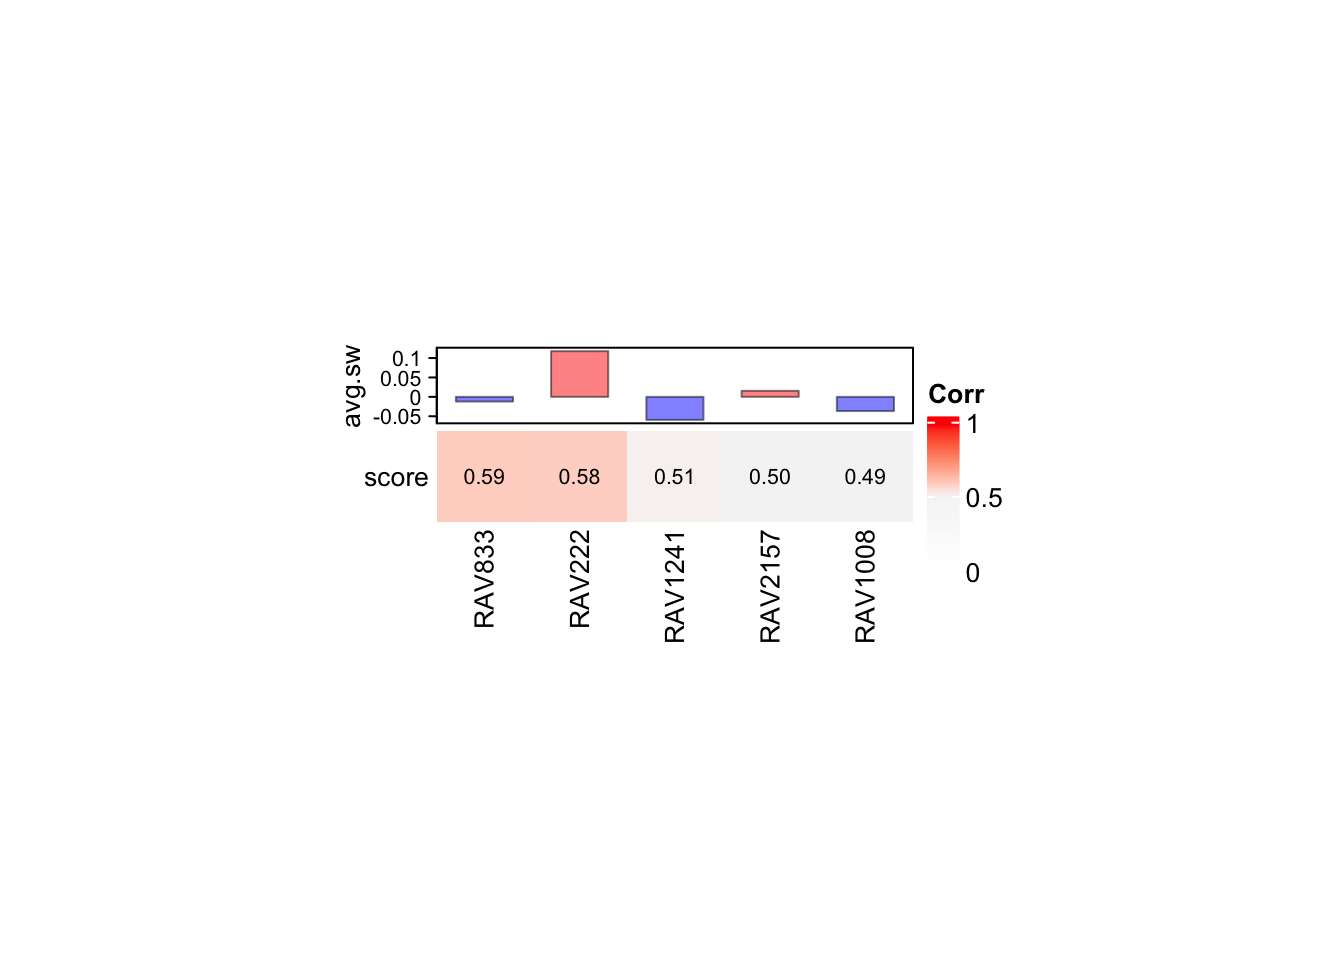
\includegraphics{EDA-COAD_files/figure-latex/unnamed-chunk-5-1.pdf}

\begin{Shaded}
\begin{Highlighting}[]
\FunctionTok{assay}\NormalTok{(coad\_rna) }\OtherTok{\textless{}{-}} \FunctionTok{log2}\NormalTok{(}\FunctionTok{assay}\NormalTok{(coad\_rna) }\SpecialCharTok{+} \DecValTok{1}\NormalTok{)}

\NormalTok{validate\_coad\_rna }\OtherTok{\textless{}{-}} \FunctionTok{validate}\NormalTok{(coad\_rna, RAVmodel)}
\FunctionTok{heatmapTable}\NormalTok{(validate\_coad\_rna, RAVmodel)}
\end{Highlighting}
\end{Shaded}

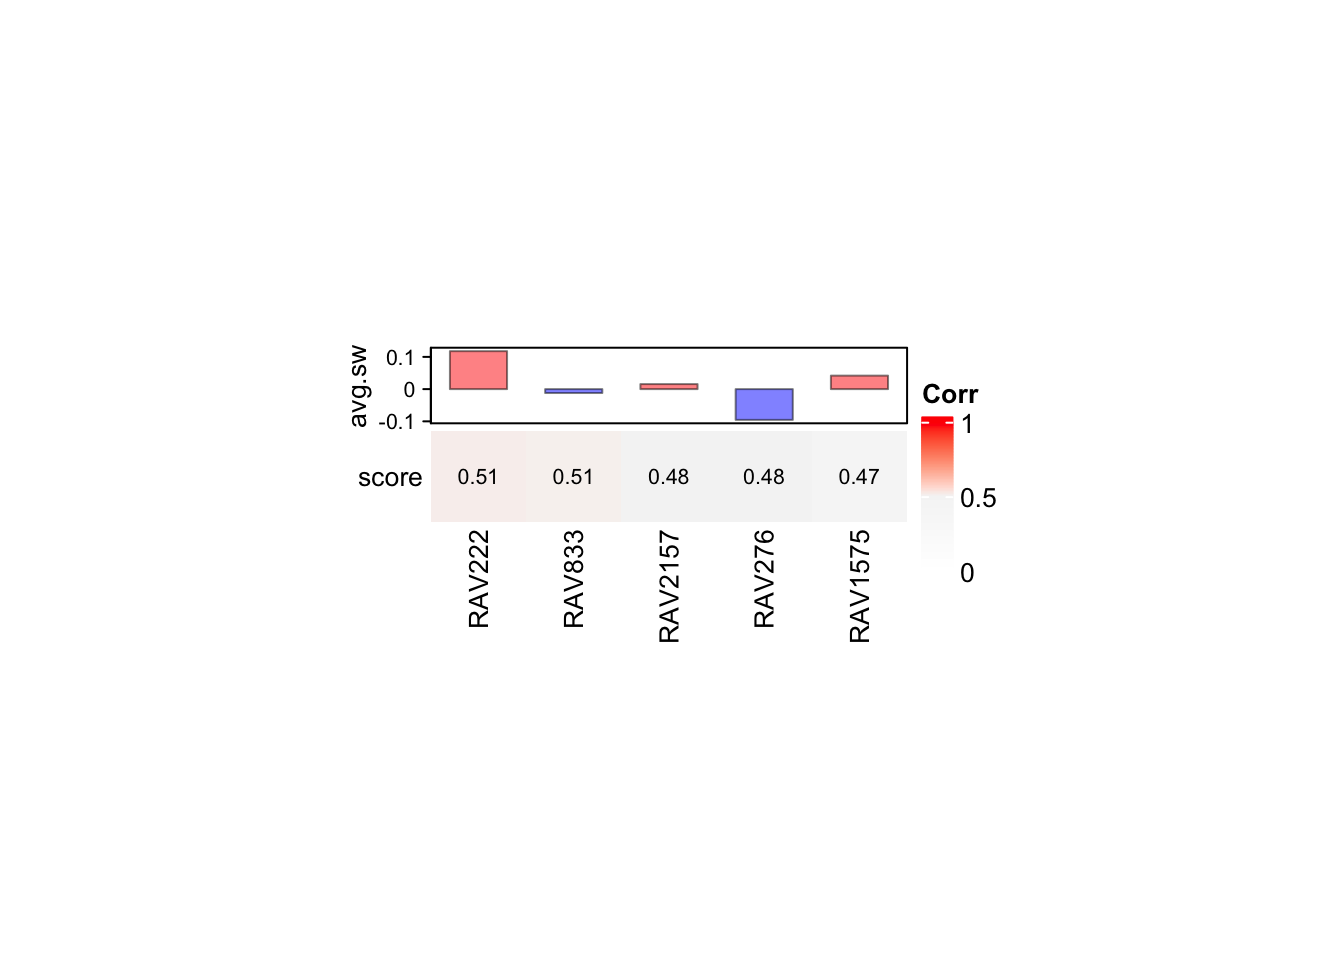
\includegraphics{EDA-COAD_files/figure-latex/unnamed-chunk-6-1.pdf} \#
Subset \#\# Filter attributes

\begin{Shaded}
\begin{Highlighting}[]
\NormalTok{sparsity\_summary }\OtherTok{\textless{}{-}} \FunctionTok{table}\NormalTok{(}\FunctionTok{colSums}\NormalTok{(}\FunctionTok{is.na}\NormalTok{(coad\_meta)))}
\NormalTok{sparsity\_summary}
\end{Highlighting}
\end{Shaded}

\begin{verbatim}
## 
##   0   1   2   3   4   5   6   7   8   9  10  12  13  14  15  20  23  24  25  27 
##  80  75   5  19  68   3   2  13   2  23   5   1   1   2  26   2   2   1   1   1 
##  30  35  37  39  41  42  43  44  48  49  52  53  55  58  59  62  63  64  65  68 
##   2  15   2   3   1  15   4   1   1   1   9   2   2   2  14   1   8   2   3   3 
##  70  72  75  76  77  78  79  81  82  85  87  88  91  97  98  99 100 101 103 106 
##   3   1   1   2   1   1   1   1   1   1   3   2   1   1   1   5   2   1   1   1 
## 107 111 120 147 172 175 185 187 195 203 206 207 208 209 212 215 216 218 220 223 
##   2   1   1   1   2   1   1   1   1   1   5   7   2   1   1   1   3   1   1   1 
## 224 225 226 231 233 236 238 239 240 244 245 246 247 250 252 253 254 255 258 259 
##   1   2   1   3   1   2  21   1   1   8   3   1   1   3   1   4   1   1  14   5 
## 260 262 263 266 268 269 270 271 272 273 274 275 276 277 278 279 280 281 282 283 
##   1   2   4   4   7   1   1  58   1   1  31  24   4  38   3  14  26   7   4  25 
## 284 285 286 287 288 289 290 291 292 293 295 296 297 298 299 300 302 303 304 305 
##   5  16   2  10   4   4   1   5   3  31  20  14   3  12   5  15  32  16   7  30 
## 306 307 308 309 310 311 312 313 314 315 316 317 318 319 320 321 322 323 324 325 
##   3  22  10   6   7  24  42  36  27   9  14  15  48 168  91  86 234 101 190 197 
## 326 
## 230
\end{verbatim}

\hypertarget{sparsity-plot}{%
\subsection{Sparsity Plot}\label{sparsity-plot}}

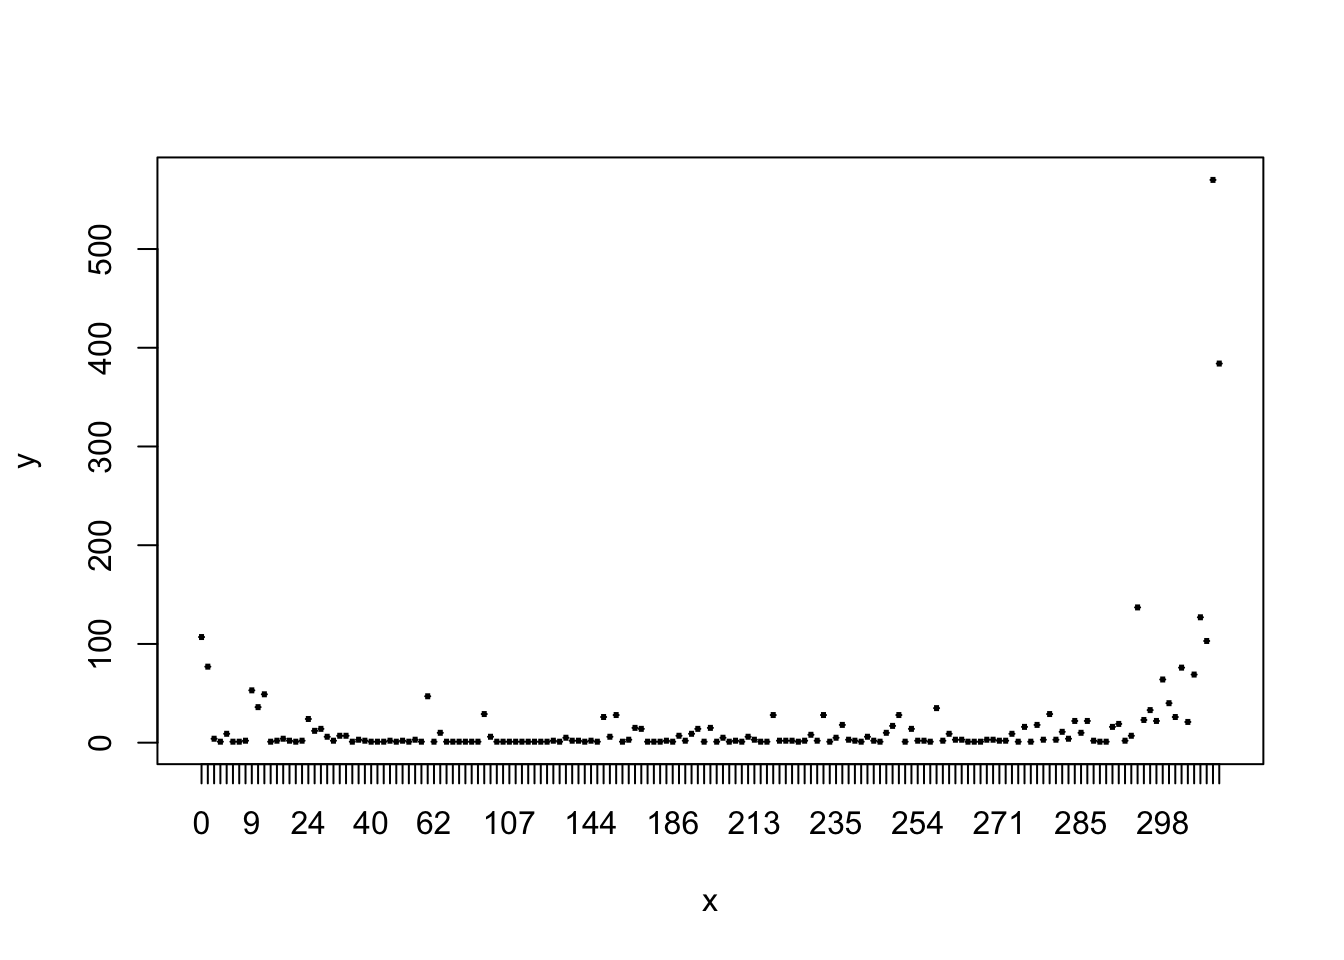
\includegraphics{EDA-COAD_files/figure-latex/unnamed-chunk-8-1.pdf}

\begin{Shaded}
\begin{Highlighting}[]
\CommentTok{\# Select columns with \textgreater{}10\% completeness}
\NormalTok{keep\_attribute\_ind }\OtherTok{\textless{}{-}} \FunctionTok{which}\NormalTok{(}\FunctionTok{colSums}\NormalTok{(}\SpecialCharTok{!}\FunctionTok{is.na}\NormalTok{(coad\_meta)) }\SpecialCharTok{\textgreater{}} \FunctionTok{round}\NormalTok{(}\FunctionTok{nrow}\NormalTok{(coad\_meta)}\SpecialCharTok{/}\DecValTok{10}\NormalTok{))}
\NormalTok{meta\_sub1 }\OtherTok{\textless{}{-}}\NormalTok{ coad\_meta[keep\_attribute\_ind]}
\NormalTok{meta\_sub1 }\OtherTok{\textless{}{-}} \FunctionTok{subset}\NormalTok{(meta\_sub1, }\AttributeTok{select=} \SpecialCharTok{{-}}\NormalTok{patientID)}
\end{Highlighting}
\end{Shaded}

\begin{Shaded}
\begin{Highlighting}[]
\CommentTok{\# Randomly select for 100 rows}
\FunctionTok{set.seed}\NormalTok{(}\DecValTok{1}\NormalTok{)}
\NormalTok{random\_sample\_ind }\OtherTok{\textless{}{-}} \FunctionTok{sample}\NormalTok{(}\DecValTok{1}\SpecialCharTok{:}\FunctionTok{nrow}\NormalTok{(meta\_sub1), }\DecValTok{100}\NormalTok{)}
\NormalTok{meta\_sub2 }\OtherTok{\textless{}{-}}\NormalTok{ meta\_sub1[random\_sample\_ind,]}
\end{Highlighting}
\end{Shaded}

\begin{Shaded}
\begin{Highlighting}[]
\CommentTok{\# Check for data types in listData}
\FunctionTok{unique}\NormalTok{(}\FunctionTok{sapply}\NormalTok{(coad\_meta}\SpecialCharTok{@}\NormalTok{listData, type))}
\end{Highlighting}
\end{Shaded}

\begin{verbatim}
## [1] "character" "integer"   "double"
\end{verbatim}

\begin{Shaded}
\begin{Highlighting}[]
\NormalTok{charcTb }\OtherTok{\textless{}{-}}\NormalTok{ meta\_sub2[, }\FunctionTok{sapply}\NormalTok{(meta\_sub1, class) }\SpecialCharTok{==} \StringTok{\textquotesingle{}character\textquotesingle{}}\NormalTok{]}
\NormalTok{numTb }\OtherTok{\textless{}{-}}\NormalTok{ meta\_sub2[, }\FunctionTok{sapply}\NormalTok{(meta\_sub1, class) }\SpecialCharTok{\%in\%} \FunctionTok{c}\NormalTok{(}\StringTok{\textquotesingle{}numeric\textquotesingle{}}\NormalTok{, }\StringTok{\textquotesingle{}integer\textquotesingle{}}\NormalTok{)]}
\end{Highlighting}
\end{Shaded}

\begin{Shaded}
\begin{Highlighting}[]
\CommentTok{\# Calculate validation scores}
\NormalTok{sampleScore }\OtherTok{\textless{}{-}} \FunctionTok{calculateScore}\NormalTok{(coad\_rna, RAVmodel)}
\end{Highlighting}
\end{Shaded}

\begin{Shaded}
\begin{Highlighting}[]
\NormalTok{validated\_ind }\OtherTok{\textless{}{-}} \FunctionTok{validatedSignatures}\NormalTok{(validate\_coad\_rna, RAVmodel, }\AttributeTok{num.out =} \DecValTok{15}\NormalTok{, }\AttributeTok{scoreCutoff =} \FloatTok{0.45}\NormalTok{, }\AttributeTok{indexOnly =} \ConstantTok{TRUE}\NormalTok{)}
\end{Highlighting}
\end{Shaded}

\begin{verbatim}
## RAV61 can be filtered based on GSEA_C2
\end{verbatim}

\begin{verbatim}
## RAV517 can be filtered based on GSEA_C2
\end{verbatim}

\begin{Shaded}
\begin{Highlighting}[]
\CommentTok{\# Subset sampleScore to join with MCPcounter}
\NormalTok{sampleScore\_sub }\OtherTok{\textless{}{-}}\NormalTok{ sampleScore[random\_sample\_ind, validated\_ind] }\SpecialCharTok{\%\textgreater{}\%} \FunctionTok{as.data.frame}\NormalTok{()}
\end{Highlighting}
\end{Shaded}

\hypertarget{calculate-r-squared-value-for-numeric-variables}{%
\section{Calculate R-Squared Value for Numeric
Variables}\label{calculate-r-squared-value-for-numeric-variables}}

\begin{Shaded}
\begin{Highlighting}[]
\CommentTok{\# R squared value function}
\NormalTok{calculateRsq }\OtherTok{\textless{}{-}} \ControlFlowTok{function}\NormalTok{ (x, y) stats}\SpecialCharTok{::}\FunctionTok{cor}\NormalTok{(x, y, }\AttributeTok{use =} \StringTok{\textquotesingle{}na.or.complete\textquotesingle{}}\NormalTok{) }\SpecialCharTok{\^{}} \DecValTok{2}
\end{Highlighting}
\end{Shaded}

\begin{Shaded}
\begin{Highlighting}[]
\CommentTok{\# Calculate r{-}squared for numeric attributes}
\NormalTok{rsq\_numAttr }\OtherTok{\textless{}{-}} \FunctionTok{as.data.frame}\NormalTok{(}\FunctionTok{matrix}\NormalTok{(}\AttributeTok{nrow =} \FunctionTok{ncol}\NormalTok{(numTb),}
                                    \AttributeTok{ncol =} \FunctionTok{ncol}\NormalTok{(sampleScore\_sub)))}

\FunctionTok{colnames}\NormalTok{(rsq\_numAttr) }\OtherTok{\textless{}{-}} \FunctionTok{colnames}\NormalTok{(sampleScore\_sub)}
\FunctionTok{rownames}\NormalTok{(rsq\_numAttr) }\OtherTok{\textless{}{-}} \FunctionTok{colnames}\NormalTok{(numTb)}

\ControlFlowTok{for}\NormalTok{ (i }\ControlFlowTok{in} \FunctionTok{seq\_len}\NormalTok{(}\FunctionTok{ncol}\NormalTok{(numTb))) \{}
  \ControlFlowTok{for}\NormalTok{ (j }\ControlFlowTok{in} \FunctionTok{seq\_len}\NormalTok{(}\FunctionTok{ncol}\NormalTok{(sampleScore\_sub))) \{}
\NormalTok{    rsq }\OtherTok{\textless{}{-}} \FunctionTok{calculateRsq}\NormalTok{(numTb[, i], sampleScore\_sub[, j])}
\NormalTok{    rsq\_numAttr[i, j] }\OtherTok{\textless{}{-}}\NormalTok{ rsq}
\NormalTok{  \}}
\NormalTok{\}}

\NormalTok{rsq\_numAttr }\OtherTok{\textless{}{-}} \FunctionTok{na.omit}\NormalTok{(rsq\_numAttr)}
\end{Highlighting}
\end{Shaded}

\begin{Shaded}
\begin{Highlighting}[]
\CommentTok{\# Remove batch effect variables}
\NormalTok{batch\_num\_ind }\OtherTok{\textless{}{-}} \FunctionTok{grep}\NormalTok{(}\StringTok{\textquotesingle{}analyte|portion|procurement|aliquot|uuid|barcode\textquotesingle{}}\NormalTok{,}
                  \FunctionTok{rownames}\NormalTok{(rsq\_numAttr))}
\NormalTok{rsq\_numAttr\_no\_batch }\OtherTok{\textless{}{-}}\NormalTok{ rsq\_numAttr[}\SpecialCharTok{{-}}\NormalTok{batch\_num\_ind,]}
\end{Highlighting}
\end{Shaded}

\begin{Shaded}
\begin{Highlighting}[]
\NormalTok{max\_rav }\OtherTok{\textless{}{-}} \FunctionTok{apply}\NormalTok{(rsq\_numAttr\_no\_batch, }\DecValTok{1}\NormalTok{, max)}
\NormalTok{max\_attr }\OtherTok{\textless{}{-}} \FunctionTok{which}\NormalTok{(max\_rav }\SpecialCharTok{\textgreater{}} \FloatTok{0.5}\NormalTok{)}

\NormalTok{target\_rsq }\OtherTok{\textless{}{-}}\NormalTok{ rsq\_numAttr\_no\_batch[max\_attr,]}
\end{Highlighting}
\end{Shaded}

\hypertarget{heatmaptable}{%
\section{heatmapTable}\label{heatmaptable}}

\begin{Shaded}
\begin{Highlighting}[]
\FunctionTok{options}\NormalTok{(}\AttributeTok{ztable.type=}\StringTok{\textquotesingle{}html\textquotesingle{}}\NormalTok{)}
\NormalTok{z }\OtherTok{=} \FunctionTok{ztable}\NormalTok{(target\_rsq)}
\NormalTok{z }\SpecialCharTok{\%\textgreater{}\%} \FunctionTok{makeHeatmap}\NormalTok{(}\AttributeTok{palette=}\StringTok{"Blues"}\NormalTok{)}
\end{Highlighting}
\end{Shaded}

~

patient.number\_of\_abnormal\_loci

0.21

0.02

0.05

0.01

0.18

0.03

0.72

0.25

0.25

0.04

0.17

0.28

0.22

0.25

0.22

patient.samples.sample.3.sample\_type\_id

0.42

0.05

0.18

0.28

0.49

0.01

0.02

0.58

0.46

0.22

0.59

0.64

0.21

0.19

0.02

WGS

0.10

0.46

0.29

0.51

0.59

0.47

0.02

0.53

0.62

0.58

0.27

0.44

0.19

0.21

0.49

age\_at\_initial\_pathologic\_diagnosis

0.06

0.02

0.04

0.10

0.06

0.01

0.57

0.08

0.01

0.05

0.22

0.14

0.01

0.22

0.05

\begin{Shaded}
\begin{Highlighting}[]
\FunctionTok{heatmap}\NormalTok{(}\FunctionTok{as.matrix}\NormalTok{(target\_rsq), }\AttributeTok{scale=}\StringTok{"column"}\NormalTok{)}
\end{Highlighting}
\end{Shaded}

\includegraphics{EDA-COAD_files/figure-latex/unnamed-chunk-18-1.pdf} \#
Separate out Factor Variables by number of levels (1, 2, 3+) not
including NA

\begin{Shaded}
\begin{Highlighting}[]
\CommentTok{\# Convert to factor data type}
\NormalTok{factorTb }\OtherTok{\textless{}{-}}\NormalTok{ meta\_sub2[, }\FunctionTok{sapply}\NormalTok{(meta\_sub1, class) }\SpecialCharTok{==} \StringTok{\textquotesingle{}character\textquotesingle{}}\NormalTok{]}

\NormalTok{factorTb[}\FunctionTok{sapply}\NormalTok{(factorTb, is.character)] }\OtherTok{\textless{}{-}} \FunctionTok{lapply}\NormalTok{(factorTb[}\FunctionTok{sapply}\NormalTok{(factorTb, is.character)], factor, }\AttributeTok{exclude =} \ConstantTok{NULL}\NormalTok{)}

\CommentTok{\#any(is.na(levels(factorTb[,2])))}
\CommentTok{\#!any(is.na(levels(factorTb[,6])))}

\NormalTok{single\_fac\_ind }\OtherTok{\textless{}{-}} \FunctionTok{c}\NormalTok{()}
\NormalTok{binary\_fac\_ind }\OtherTok{\textless{}{-}} \FunctionTok{c}\NormalTok{()}
\NormalTok{multi\_fac\_ind }\OtherTok{\textless{}{-}} \FunctionTok{c}\NormalTok{()}

\CommentTok{\# Testing factor grouping}
\ControlFlowTok{for}\NormalTok{ (i }\ControlFlowTok{in} \DecValTok{1}\SpecialCharTok{:}\FunctionTok{length}\NormalTok{(factorTb)) \{}
  \ControlFlowTok{if}\NormalTok{ (}\FunctionTok{nlevels}\NormalTok{(factorTb[,i]) }\SpecialCharTok{==} \DecValTok{1} \SpecialCharTok{|} 
\NormalTok{      (}\FunctionTok{nlevels}\NormalTok{(factorTb[,i]) }\SpecialCharTok{==} \DecValTok{2} \SpecialCharTok{\&} 
       \FunctionTok{any}\NormalTok{(}\FunctionTok{is.na}\NormalTok{(}\FunctionTok{levels}\NormalTok{(factorTb[,i]))))}
\NormalTok{      ) \{}
\NormalTok{    single\_fac\_ind }\OtherTok{\textless{}{-}} \FunctionTok{c}\NormalTok{(single\_fac\_ind, i)}
\NormalTok{  \} }\ControlFlowTok{else} \ControlFlowTok{if}\NormalTok{ (}\CommentTok{\#nlevels(factorTb[,i]) == 3 \& }
             \CommentTok{\#any(is.na(levels(factorTb[,i]))) |}
             
\NormalTok{             (}\FunctionTok{nlevels}\NormalTok{(factorTb[,i]) }\SpecialCharTok{==} \DecValTok{2} \SpecialCharTok{\&} 
              \SpecialCharTok{!}\FunctionTok{any}\NormalTok{(}\FunctionTok{is.na}\NormalTok{(}\FunctionTok{levels}\NormalTok{(factorTb[,i]))))}
\NormalTok{          ) \{}
\NormalTok{    binary\_fac\_ind }\OtherTok{\textless{}{-}} \FunctionTok{c}\NormalTok{(binary\_fac\_ind, i)}
\NormalTok{  \} }\ControlFlowTok{else}\NormalTok{ \{}
\NormalTok{    multi\_fac\_ind }\OtherTok{\textless{}{-}} \FunctionTok{c}\NormalTok{(multi\_fac\_ind, i)}
\NormalTok{  \}}
\NormalTok{\}}

\NormalTok{new\_factorTb }\OtherTok{\textless{}{-}}\NormalTok{ factorTb[,multi\_fac\_ind]}
\NormalTok{binary\_factor }\OtherTok{\textless{}{-}}\NormalTok{ factorTb[,binary\_fac\_ind]}
\NormalTok{binary\_factor }\OtherTok{\textless{}{-}}\NormalTok{ binary\_factor[}\SpecialCharTok{{-}}\FunctionTok{c}\NormalTok{(}\DecValTok{7}\NormalTok{,}\DecValTok{8}\NormalTok{)]}
\NormalTok{single\_factor }\OtherTok{\textless{}{-}}\NormalTok{ factorTb[,single\_fac\_ind]}
\end{Highlighting}
\end{Shaded}

\hypertarget{calculate-f-statistic-anova-for-character-variables}{%
\section{Calculate F-statistic (ANOVA) for Character
Variables}\label{calculate-f-statistic-anova-for-character-variables}}

\begin{Shaded}
\begin{Highlighting}[]
\NormalTok{aov\_res }\OtherTok{\textless{}{-}} \FunctionTok{as.data.frame}\NormalTok{(}\FunctionTok{matrix}\NormalTok{(}\AttributeTok{nrow =} \FunctionTok{ncol}\NormalTok{(new\_factorTb),}
                                \AttributeTok{ncol =} \FunctionTok{ncol}\NormalTok{(sampleScore\_sub)))}

\FunctionTok{rownames}\NormalTok{(aov\_res) }\OtherTok{\textless{}{-}} \FunctionTok{colnames}\NormalTok{(new\_factorTb)}
\FunctionTok{colnames}\NormalTok{(aov\_res) }\OtherTok{\textless{}{-}} \FunctionTok{colnames}\NormalTok{(sampleScore\_sub)}

\NormalTok{aov\_coad\_fvalue }\OtherTok{\textless{}{-}}\NormalTok{ aov\_res}
\NormalTok{aov\_coad\_pvalue }\OtherTok{\textless{}{-}}\NormalTok{ aov\_res}

\ControlFlowTok{for}\NormalTok{ (i }\ControlFlowTok{in} \FunctionTok{seq\_len}\NormalTok{(}\FunctionTok{ncol}\NormalTok{(sampleScore\_sub))) \{}
  \ControlFlowTok{for}\NormalTok{ (j }\ControlFlowTok{in} \FunctionTok{seq\_len}\NormalTok{(}\FunctionTok{ncol}\NormalTok{(new\_factorTb))) \{}
    
    \DocumentationTok{\#\# ANOVA}
\NormalTok{    aov }\OtherTok{\textless{}{-}} \FunctionTok{aov}\NormalTok{(sampleScore\_sub[, i] }\SpecialCharTok{\textasciitilde{}}\NormalTok{ new\_factorTb[, j])}
    
    \DocumentationTok{\#\# F{-}statistic}
\NormalTok{    fval }\OtherTok{\textless{}{-}} \FunctionTok{summary}\NormalTok{(aov)[[}\DecValTok{1}\NormalTok{]]}\SpecialCharTok{$}\StringTok{\textasciigrave{}}\AttributeTok{F value}\StringTok{\textasciigrave{}}\NormalTok{[}\DecValTok{1}\NormalTok{]}
\NormalTok{    aov\_coad\_fvalue[j, i] }\OtherTok{\textless{}{-}}\NormalTok{ fval}
    
    \DocumentationTok{\#\# p{-}value}
\NormalTok{    pval }\OtherTok{\textless{}{-}} \FunctionTok{summary}\NormalTok{(aov)[[}\DecValTok{1}\NormalTok{]]}\SpecialCharTok{$}\StringTok{\textasciigrave{}}\AttributeTok{Pr(\textgreater{}F)}\StringTok{\textasciigrave{}}\NormalTok{[}\DecValTok{1}\NormalTok{]}
\NormalTok{    aov\_coad\_pvalue[j, i] }\OtherTok{\textless{}{-}}\NormalTok{ pval}
\NormalTok{  \}}
\NormalTok{\}}
\end{Highlighting}
\end{Shaded}

\begin{Shaded}
\begin{Highlighting}[]
\CommentTok{\# Select for p{-}values \textless{} 0.01}
\NormalTok{min\_rav }\OtherTok{\textless{}{-}} \FunctionTok{apply}\NormalTok{(aov\_coad\_pvalue, }\DecValTok{1}\NormalTok{, min)}
\NormalTok{min\_attr }\OtherTok{\textless{}{-}} \FunctionTok{which}\NormalTok{(min\_rav }\SpecialCharTok{\textless{}} \FloatTok{0.01}\NormalTok{)}

\NormalTok{target\_coad\_aov\_fvalue }\OtherTok{\textless{}{-}}\NormalTok{ aov\_coad\_fvalue[min\_attr,]}
\NormalTok{target\_coad\_aov\_pvalue }\OtherTok{\textless{}{-}}\NormalTok{ aov\_coad\_pvalue[min\_attr,]}
\end{Highlighting}
\end{Shaded}

\begin{Shaded}
\begin{Highlighting}[]
\NormalTok{batch\_char\_ind }\OtherTok{\textless{}{-}} \FunctionTok{grep}\NormalTok{(}\StringTok{\textquotesingle{}analyte|portion|procurement|aliquot|uuid|barcode\textquotesingle{}}\NormalTok{,}
                       \FunctionTok{rownames}\NormalTok{(target\_coad\_aov\_fvalue))}
\NormalTok{coad\_aov\_fvalue }\OtherTok{\textless{}{-}}\NormalTok{ target\_coad\_aov\_fvalue[}\SpecialCharTok{{-}}\NormalTok{batch\_char\_ind,]}
\NormalTok{coad\_aov\_pvalue }\OtherTok{\textless{}{-}}\NormalTok{ target\_coad\_aov\_pvalue[}\SpecialCharTok{{-}}\NormalTok{batch\_char\_ind,]}
\end{Highlighting}
\end{Shaded}

\begin{Shaded}
\begin{Highlighting}[]
\FunctionTok{heatmap}\NormalTok{(}\FunctionTok{as.matrix}\NormalTok{(coad\_aov\_fvalue), }\AttributeTok{main =} \StringTok{\textquotesingle{}COAD F{-}Statistics\textquotesingle{}}\NormalTok{)}
\end{Highlighting}
\end{Shaded}

\includegraphics{EDA-COAD_files/figure-latex/unnamed-chunk-23-1.pdf}

\begin{Shaded}
\begin{Highlighting}[]
\NormalTok{sig\_fval }\OtherTok{\textless{}{-}} \FunctionTok{as.data.frame}\NormalTok{(}\FunctionTok{matrix}\NormalTok{(}\AttributeTok{nrow =} \FunctionTok{ncol}\NormalTok{(new\_factorTb),}
                                \AttributeTok{ncol =} \FunctionTok{ncol}\NormalTok{(sampleScore\_sub)))}

\FunctionTok{rownames}\NormalTok{(sig\_fval) }\OtherTok{\textless{}{-}} \FunctionTok{colnames}\NormalTok{(new\_factorTb)}
\FunctionTok{colnames}\NormalTok{(sig\_fval) }\OtherTok{\textless{}{-}} \FunctionTok{colnames}\NormalTok{(sampleScore\_sub)}

\ControlFlowTok{for}\NormalTok{ (i }\ControlFlowTok{in} \FunctionTok{seq\_len}\NormalTok{(}\FunctionTok{ncol}\NormalTok{(sampleScore\_sub))) \{}
  \ControlFlowTok{for}\NormalTok{ (j }\ControlFlowTok{in} \FunctionTok{seq\_len}\NormalTok{(}\FunctionTok{ncol}\NormalTok{(new\_factorTb))) \{}
    
    \ControlFlowTok{if}\NormalTok{ (}\SpecialCharTok{!}\FunctionTok{is.null}\NormalTok{(}\FunctionTok{summary}\NormalTok{(}\FunctionTok{aov}\NormalTok{(sampleScore\_sub[, i] }\SpecialCharTok{\textasciitilde{}}\NormalTok{ new\_factorTb[, j]))[[}\DecValTok{1}\NormalTok{]]}\SpecialCharTok{$}\StringTok{\textasciigrave{}}\AttributeTok{Pr(\textgreater{}F)}\StringTok{\textasciigrave{}}\NormalTok{[}\DecValTok{1}\NormalTok{])) \{}
      
      \ControlFlowTok{if}\NormalTok{ (}\SpecialCharTok{!}\FunctionTok{is.null}\NormalTok{(}\FunctionTok{summary}\NormalTok{(}\FunctionTok{aov}\NormalTok{(sampleScore\_sub[, i] }\SpecialCharTok{\textasciitilde{}}\NormalTok{ new\_factorTb[, j]))[[}\DecValTok{1}\NormalTok{]]}\SpecialCharTok{$}\StringTok{\textasciigrave{}}\AttributeTok{F value}\StringTok{\textasciigrave{}}\NormalTok{[}\DecValTok{1}\NormalTok{]) }\SpecialCharTok{\&}
\NormalTok{          (}\FunctionTok{summary}\NormalTok{(}\FunctionTok{aov}\NormalTok{(sampleScore\_sub[, i] }\SpecialCharTok{\textasciitilde{}}\NormalTok{ new\_factorTb[, j]))[[}\DecValTok{1}\NormalTok{]]}\SpecialCharTok{$}\StringTok{\textasciigrave{}}\AttributeTok{Pr(\textgreater{}F)}\StringTok{\textasciigrave{}}\NormalTok{[}\DecValTok{1}\NormalTok{] }\SpecialCharTok{\textless{}} \FloatTok{0.05}\NormalTok{)) \{}
\NormalTok{        sig\_fval[j, i] }\OtherTok{\textless{}{-}} \FunctionTok{summary}\NormalTok{(}\FunctionTok{aov}\NormalTok{(sampleScore\_sub[, i] }\SpecialCharTok{\textasciitilde{}}\NormalTok{ new\_factorTb[, j]))[[}\DecValTok{1}\NormalTok{]]}\SpecialCharTok{$}\StringTok{\textasciigrave{}}\AttributeTok{F value}\StringTok{\textasciigrave{}}\NormalTok{[}\DecValTok{1}\NormalTok{]}
\NormalTok{      \} }\ControlFlowTok{else}\NormalTok{ \{}
        \ControlFlowTok{next}
\NormalTok{      \}}
\NormalTok{    \} }\ControlFlowTok{else}\NormalTok{ \{}
      \ControlFlowTok{next}
\NormalTok{    \}}
\NormalTok{  \}}
\NormalTok{\}}

\NormalTok{fstat\_ind }\OtherTok{\textless{}{-}} \FunctionTok{c}\NormalTok{()}

\ControlFlowTok{for}\NormalTok{ (i }\ControlFlowTok{in} \FunctionTok{seq\_len}\NormalTok{(}\FunctionTok{nrow}\NormalTok{(sig\_fval))) \{}
  \ControlFlowTok{if}\NormalTok{ (}\FunctionTok{sum}\NormalTok{(}\FunctionTok{is.na}\NormalTok{(sig\_fval[i, ])) }\SpecialCharTok{\textless{}} \DecValTok{220}\NormalTok{) \{}
\NormalTok{    fstat\_ind }\OtherTok{\textless{}{-}} \FunctionTok{c}\NormalTok{(fstat\_ind, i)}
\NormalTok{  \} }\ControlFlowTok{else}\NormalTok{ \{}
    \ControlFlowTok{next}
\NormalTok{  \}}
\NormalTok{\}}

\NormalTok{sig\_fval }\OtherTok{\textless{}{-}}\NormalTok{ sig\_fval[fstat\_ind,]}
\NormalTok{batch\_char\_ind\_2 }\OtherTok{\textless{}{-}} \FunctionTok{grep}\NormalTok{(}\StringTok{\textquotesingle{}analyte|portion|procurement|aliquot|uuid|barcode\textquotesingle{}}\NormalTok{,}
                  \FunctionTok{rownames}\NormalTok{(sig\_fval))}
\NormalTok{sig\_fval }\OtherTok{\textless{}{-}}\NormalTok{ sig\_fval[}\SpecialCharTok{{-}}\NormalTok{batch\_char\_ind\_2,]}
\end{Highlighting}
\end{Shaded}

\begin{Shaded}
\begin{Highlighting}[]
\FunctionTok{options}\NormalTok{(}\AttributeTok{ztable.type=}\StringTok{\textquotesingle{}html\textquotesingle{}}\NormalTok{)}
\CommentTok{\#ztable(sig\_fval) \%\textgreater{}\%}
 \CommentTok{\# makeHeatmap(palette = \textquotesingle{}Blues\textquotesingle{}) \#\%\textgreater{}\%}
  \CommentTok{\#print(caption=\textquotesingle{}ANOVA F{-}stats with p{-}values \textless{} 0.01\textquotesingle{})}
\end{Highlighting}
\end{Shaded}

\hypertarget{calculate-t-test-for-binomial-character-variables}{%
\section{Calculate t-test for binomial Character
Variables}\label{calculate-t-test-for-binomial-character-variables}}

\begin{Shaded}
\begin{Highlighting}[]
\CommentTok{\#Remove factors without enough y{-}observations}
\ControlFlowTok{for}\NormalTok{ (i }\ControlFlowTok{in} \FunctionTok{seq\_len}\NormalTok{(}\FunctionTok{ncol}\NormalTok{(binary\_factor))) \{}
\NormalTok{  x }\OtherTok{\textless{}{-}} \FunctionTok{summary}\NormalTok{(binary\_factor[,i])}
  
  \ControlFlowTok{if}\NormalTok{ (}\FunctionTok{all}\NormalTok{(x }\SpecialCharTok{\textgreater{}} \DecValTok{1}\NormalTok{)) \{}
    \FunctionTok{print}\NormalTok{(x)}
\NormalTok{  \} }\ControlFlowTok{else}\NormalTok{ \{}
    \FunctionTok{print}\NormalTok{(}\FunctionTok{paste}\NormalTok{(}\StringTok{"index"}\NormalTok{, i, }\StringTok{"does not have enough observations"}\NormalTok{))}
\NormalTok{  \}}
\NormalTok{\}}
\end{Highlighting}
\end{Shaded}

\begin{verbatim}
## female   male 
##     52     48 
##          colon adenocarcinoma colon mucinous adenocarcinoma 
##                            92                             8 
## consented  deceased 
##        91         9 
##          colon adenocarcinoma colon mucinous adenocarcinoma 
##                            92                             8 
## [1] "index 5 does not have enough observations"
## female   male 
##     52     48 
## alive  dead 
##    87    13 
##        canonical canonical - plus 
##               69               31 
## consented  deceased 
##        91         9 
##  no yes 
##  94   6 
##          colon adenocarcinoma colon mucinous adenocarcinoma 
##                            92                             8 
## [1] "index 12 does not have enough observations"
##  no yes 
##   7  93 
##  no yes 
##  14  86 
##  no yes 
##  96   4 
##  no yes 
##  96   4 
##  no yes 
##  96   4 
##  no yes 
##  81  19 
##  no yes 
##  96   4 
## picogreen   uv spec 
##        17        83 
##  no yes 
##  96   4 
##  a  b 
## 95  5 
##  no yes 
##  76  24 
## picogreen   uv spec 
##        13        87 
## bottom    top 
##     67     33 
## [1] "index 26 does not have enough observations"
\end{verbatim}

\begin{Shaded}
\begin{Highlighting}[]
\NormalTok{bin\_fac }\OtherTok{\textless{}{-}}\NormalTok{ binary\_factor[,}\SpecialCharTok{{-}}\FunctionTok{c}\NormalTok{(}\DecValTok{5}\NormalTok{, }\DecValTok{12}\NormalTok{, }\DecValTok{26}\NormalTok{)]}

\NormalTok{t\_test\_res }\OtherTok{\textless{}{-}} \FunctionTok{as.data.frame}\NormalTok{(}\FunctionTok{matrix}\NormalTok{(}\AttributeTok{nrow =} \FunctionTok{ncol}\NormalTok{(bin\_fac),}
                                \AttributeTok{ncol =} \FunctionTok{ncol}\NormalTok{(sampleScore\_sub)))}

\FunctionTok{rownames}\NormalTok{(t\_test\_res) }\OtherTok{\textless{}{-}} \FunctionTok{colnames}\NormalTok{(bin\_fac)}
\FunctionTok{colnames}\NormalTok{(t\_test\_res) }\OtherTok{\textless{}{-}} \FunctionTok{colnames}\NormalTok{(sampleScore\_sub)}

\NormalTok{ttest\_coad\_tvalue }\OtherTok{\textless{}{-}}\NormalTok{ t\_test\_res}
\NormalTok{ttest\_coad\_pvalue }\OtherTok{\textless{}{-}}\NormalTok{ t\_test\_res}

\ControlFlowTok{for}\NormalTok{ (i }\ControlFlowTok{in} \FunctionTok{seq\_len}\NormalTok{(}\FunctionTok{ncol}\NormalTok{(sampleScore\_sub))) \{}
  \ControlFlowTok{for}\NormalTok{ (j }\ControlFlowTok{in} \FunctionTok{seq\_len}\NormalTok{(}\FunctionTok{ncol}\NormalTok{(bin\_fac))) \{}
    
    \DocumentationTok{\#\# t{-}test}
\NormalTok{      t\_test }\OtherTok{\textless{}{-}} \FunctionTok{t.test}\NormalTok{(sampleScore\_sub[, i] }\SpecialCharTok{\textasciitilde{}}\NormalTok{ bin\_fac[,j])}
    
    \DocumentationTok{\#\# t{-}value}
\NormalTok{      tval }\OtherTok{\textless{}{-}}\NormalTok{ t\_test}\SpecialCharTok{$}\NormalTok{statistic}
\NormalTok{      ttest\_coad\_tvalue[j, i] }\OtherTok{\textless{}{-}}\NormalTok{ tval}
    
    \DocumentationTok{\#\# p{-}value}
\NormalTok{      pval }\OtherTok{\textless{}{-}}\NormalTok{ t\_test}\SpecialCharTok{$}\NormalTok{p.val}
\NormalTok{      ttest\_coad\_pvalue[j, i] }\OtherTok{\textless{}{-}}\NormalTok{ pval}
\NormalTok{  \}}
\NormalTok{\}}

\NormalTok{batch\_char\_ind }\OtherTok{\textless{}{-}} \FunctionTok{grep}\NormalTok{(}\StringTok{\textquotesingle{}analyte|portion|procurement|aliquot|uuid|barcode\textquotesingle{}}\NormalTok{,}
                  \FunctionTok{rownames}\NormalTok{(ttest\_coad\_tvalue))}
\NormalTok{ttest\_coad\_tvalue\_2 }\OtherTok{\textless{}{-}}\NormalTok{ ttest\_coad\_tvalue[}\SpecialCharTok{{-}}\NormalTok{batch\_char\_ind,]}
\end{Highlighting}
\end{Shaded}

\begin{Shaded}
\begin{Highlighting}[]
\FunctionTok{heatmap}\NormalTok{(}\FunctionTok{as.matrix}\NormalTok{(ttest\_coad\_tvalue\_2), }\AttributeTok{main =} \StringTok{\textquotesingle{}COAD T{-}Test\textquotesingle{}}\NormalTok{)}
\end{Highlighting}
\end{Shaded}

\includegraphics{EDA-COAD_files/figure-latex/unnamed-chunk-27-1.pdf}

\begin{Shaded}
\begin{Highlighting}[]
\CommentTok{\#Only view t{-}values with significant p{-}value (\textless{}0.05)}
\NormalTok{ttest\_coad\_sig\_tvalue }\OtherTok{\textless{}{-}}\NormalTok{ t\_test\_res}


 \ControlFlowTok{for}\NormalTok{ (i }\ControlFlowTok{in} \FunctionTok{seq\_len}\NormalTok{(}\FunctionTok{ncol}\NormalTok{(sampleScore\_sub))) \{}
   \ControlFlowTok{for}\NormalTok{ (j }\ControlFlowTok{in} \FunctionTok{seq\_len}\NormalTok{(}\FunctionTok{ncol}\NormalTok{(bin\_fac))) \{}
     \ControlFlowTok{if}\NormalTok{ (}\FunctionTok{t.test}\NormalTok{(sampleScore\_sub[, i] }\SpecialCharTok{\textasciitilde{}}\NormalTok{ bin\_fac[,j])}\SpecialCharTok{$}\NormalTok{p.val }\SpecialCharTok{\textless{}} \FloatTok{0.05}\NormalTok{) \{}
\NormalTok{       ttest\_coad\_sig\_tvalue[j, i] }\OtherTok{\textless{}{-}} \FunctionTok{t.test}\NormalTok{(sampleScore\_sub[, i] }\SpecialCharTok{\textasciitilde{}}\NormalTok{ bin\_fac[,j])}\SpecialCharTok{$}\NormalTok{statistic}
\NormalTok{     \}}
\NormalTok{   \}}
\NormalTok{ \}}

\NormalTok{batch\_char\_ind }\OtherTok{\textless{}{-}} \FunctionTok{grep}\NormalTok{(}\StringTok{\textquotesingle{}analyte|portion|procurement|aliquot|uuid|barcode\textquotesingle{}}\NormalTok{,}
                  \FunctionTok{rownames}\NormalTok{(ttest\_coad\_sig\_tvalue))}
\NormalTok{ttest\_coad\_sig\_tvalue }\OtherTok{\textless{}{-}}\NormalTok{ ttest\_coad\_sig\_tvalue[}\SpecialCharTok{{-}}\NormalTok{batch\_char\_ind,]}
\end{Highlighting}
\end{Shaded}

\begin{Shaded}
\begin{Highlighting}[]
\FunctionTok{options}\NormalTok{(}\AttributeTok{ztable.type=}\StringTok{\textquotesingle{}html\textquotesingle{}}\NormalTok{)}
\FunctionTok{ztable}\NormalTok{(ttest\_coad\_sig\_tvalue) }\SpecialCharTok{\%\textgreater{}\%}
  \FunctionTok{makeHeatmap}\NormalTok{(}\AttributeTok{palette =} \StringTok{\textquotesingle{}Blues\textquotesingle{}}\NormalTok{) }\SpecialCharTok{\%\textgreater{}\%}
  \FunctionTok{print}\NormalTok{(}\AttributeTok{caption=}\StringTok{\textquotesingle{}T{-}test with p{-}values \textless{} 0.05\textquotesingle{}}\NormalTok{)}
\end{Highlighting}
\end{Shaded}

T-test with p-values \textless{} 0.05

~

gender.x

NA

histological\_type.x

-3.49

-2.85

3.32

NA

-3.55

2.32

-3.27

3.58

2.52

patient.clinical\_cqcf.consent\_or\_death\_status

NA

3.52

-3.26

patient.clinical\_cqcf.histological\_type

-3.49

-2.85

3.32

NA

-3.55

2.32

-3.27

3.58

2.52

patient.gender

NA

patient.vital\_status

NA

2.23

patient.bcr\_canonical\_check.bcr\_patient\_canonical\_status

5.23

-2.73

3.63

-3.09

NA

-2.23

2.02

2.82

3.12

-3.60

patient.biospecimen\_cqcf.consent\_or\_death\_status

NA

3.52

-3.26

patient.biospecimen\_cqcf.digital\_image\_submitted

-3.46

NA

patient.biospecimen\_cqcf.histological\_type

-3.49

-2.85

3.32

NA

-3.55

2.32

-3.27

3.58

2.52

patient.biospecimen\_cqcf.path\_confirm\_report\_attached

3.95

2.94

-3.61

3.08

NA

3.53

-2.98

3.92

-2.87

-4.01

patient.biospecimen\_cqcf.top\_slide\_submitted

-2.72

-2.43

2.21

NA

patient.samples.sample.2.is\_ffpe

10.63

-2.97

NA

3.69

-3.96

-3.41

patient.samples.sample.2.vial\_number

NA

\hypertarget{rav-exploration}{%
\subsection{RAV Exploration}\label{rav-exploration}}

\begin{Shaded}
\begin{Highlighting}[]
\NormalTok{ind }\OtherTok{\textless{}{-}} \DecValTok{833}
\FunctionTok{findStudiesInCluster}\NormalTok{(RAVmodel, ind, }\AttributeTok{studyTitle =} \ConstantTok{TRUE}\NormalTok{)}
\end{Highlighting}
\end{Shaded}

\begin{verbatim}
##   studyName PC Variance explained (%)
## 1 SRP010181  3                   3.88
## 2 SRP094781  9                   2.28
## 3 SRP101290  3                   2.34
## 4 SRP148497  2                   7.61
## 5 SRP152577  3                   2.74
## 6 SRP172499  3                   6.93
##                                                                                                                                       title
## 1                                                                                    Derivation of HLA types from shotgun sequence datasets
## 2                           Molecular portraits of tumor mutational and micro-environmental sculpting by immune checkpoint blockade therapy
## 3 Tracing the temporal-spatial transcriptomic landscapes of the human fetal digestive tract by single cell RNA-seq analysis [fetal tissues]
## 4                                                                         Prediction Model of Recurrence in Endometrioid Endometrial Cancer
## 5                                                             PyMINEr Finds Gene and Autocrine/Paracrine Networks from Human Islet scRNAseq
## 6                                                                        Proteogenomic characterization of human early-onset gastric cancer
\end{verbatim}

\begin{Shaded}
\begin{Highlighting}[]
\FunctionTok{drawWordcloud}\NormalTok{(RAVmodel, ind)}
\end{Highlighting}
\end{Shaded}

\begin{verbatim}
## Warning in wordcloud::wordcloud(words = all$word, freq = all$freq, scale =
## scale, : Stomach Neoplasms could not be fit on page. It will not be plotted.
\end{verbatim}

\begin{verbatim}
## Warning in wordcloud::wordcloud(words = all$word, freq = all$freq, scale =
## scale, : Histocompatibility Antigens Class II could not be fit on page. It will
## not be plotted.
\end{verbatim}

\includegraphics{EDA-COAD_files/figure-latex/unnamed-chunk-30-1.pdf}

\begin{Shaded}
\begin{Highlighting}[]
\CommentTok{\# sampleScore1 \textless{}{-} 1001}
\CommentTok{\# sampleScore2 \textless{}{-} 1002}
\CommentTok{\# }
\CommentTok{\# plot\_data \textless{}{-} sampleScore\_sub[, c("RAV1001", "RAV1002")]}
\CommentTok{\# colnames(plot\_data)[1] \textless{}{-} "sampleScore1"}
\CommentTok{\# colnames(plot\_data)[2] \textless{}{-} "sampleScore2"}
\CommentTok{\# }
\CommentTok{\# plot\_data \textless{}{-} data.frame(plot\_data, binary\_factor)}
\CommentTok{\# }
\CommentTok{\# colors \textless{}{-} gg\_color\_hue(length(unique(plot\_data$patient.gender}
\CommentTok{\# )))}
\CommentTok{\# colors.toplot \textless{}{-} c(colors, "gray")}
\CommentTok{\# }
\CommentTok{\# pA \textless{}{-} ggplot(plot\_data,}
\CommentTok{\#              aes(x = sampleScore1, y = sampleScore2, color = patient.gender}
\CommentTok{\# )) +}
\CommentTok{\#   geom\_point() +}
\CommentTok{\#   ggtitle(\textquotesingle{}Score Plot for Gender\textquotesingle{}) +}
\CommentTok{\#   scale\_color\_manual(values = colors.toplot, name = "Gender") +}
\CommentTok{\#   theme\_bw() +}
\CommentTok{\#   theme(panel.grid.major = element\_blank(),}
\CommentTok{\#         panel.grid.minor = element\_blank()) +}
\CommentTok{\#   geom\_hline(yintercept = 0, linetype = \textquotesingle{}dashed\textquotesingle{}) +}
\CommentTok{\#   geom\_vline(xintercept = 0, linetype = \textquotesingle{}dashed\textquotesingle{}) +}
\CommentTok{\#   xlab(paste0("RAV", sampleScore1)) + ylab(paste0("RAV", sampleScore2))}
\CommentTok{\# }
\CommentTok{\# print(pA)}
\end{Highlighting}
\end{Shaded}

\begin{Shaded}
\begin{Highlighting}[]
\CommentTok{\# Function to Display Categorical Attributes\textquotesingle{} Score Plots}

\NormalTok{graph\_categorical }\OtherTok{\textless{}{-}} \ControlFlowTok{function}\NormalTok{(rav1, rav2, c, d, }\AttributeTok{e =} \StringTok{\textquotesingle{}Legend\textquotesingle{}}\NormalTok{) \{}
\NormalTok{  sampleScore1 }\OtherTok{\textless{}{-}} \FunctionTok{paste0}\NormalTok{(}\StringTok{\textquotesingle{}RAV\textquotesingle{}}\NormalTok{, rav1)}
\NormalTok{  sampleScore2 }\OtherTok{\textless{}{-}} \FunctionTok{paste0}\NormalTok{(}\StringTok{\textquotesingle{}RAV\textquotesingle{}}\NormalTok{, rav2)}

\NormalTok{  plot\_data }\OtherTok{\textless{}{-}}\NormalTok{ sampleScore\_sub[, }\FunctionTok{c}\NormalTok{(sampleScore1, sampleScore2)]}
  \FunctionTok{colnames}\NormalTok{(plot\_data)[}\DecValTok{1}\NormalTok{] }\OtherTok{\textless{}{-}} \StringTok{"sampleScore1"}
  \FunctionTok{colnames}\NormalTok{(plot\_data)[}\DecValTok{2}\NormalTok{] }\OtherTok{\textless{}{-}} \StringTok{"sampleScore2"}

\NormalTok{  plot\_data }\OtherTok{\textless{}{-}} \FunctionTok{data.frame}\NormalTok{(plot\_data, d)}
\NormalTok{  plot\_data\_2 }\OtherTok{\textless{}{-}}\NormalTok{ plot\_data[}\FunctionTok{which}\NormalTok{(}\SpecialCharTok{!}\FunctionTok{is.na}\NormalTok{(}\FunctionTok{factor}\NormalTok{(plot\_data[[c]]))),]}

\NormalTok{  colors }\OtherTok{\textless{}{-}} \FunctionTok{gg\_color\_hue}\NormalTok{(}\FunctionTok{length}\NormalTok{(}\FunctionTok{unique}\NormalTok{(plot\_data\_2[[c]])))}
\NormalTok{  colors.toplot }\OtherTok{\textless{}{-}} \FunctionTok{c}\NormalTok{(colors)}

\NormalTok{  pA }\OtherTok{\textless{}{-}} \FunctionTok{ggplot}\NormalTok{(plot\_data\_2,}
             \FunctionTok{aes}\NormalTok{(}\AttributeTok{x =}\NormalTok{ sampleScore1, }\AttributeTok{y =}\NormalTok{ sampleScore2, }\AttributeTok{color =}\NormalTok{ plot\_data\_2[[c]]}
\NormalTok{                 )) }\SpecialCharTok{+}
        \FunctionTok{geom\_point}\NormalTok{() }\SpecialCharTok{+}
        \CommentTok{\#ggtitle(\textquotesingle{}Score Plot for Gender\textquotesingle{}) +}
        \FunctionTok{scale\_color\_manual}\NormalTok{(}\AttributeTok{values =}\NormalTok{ colors.toplot, }\AttributeTok{name =}\NormalTok{ e) }\SpecialCharTok{+}
        \FunctionTok{theme\_bw}\NormalTok{() }\SpecialCharTok{+}
        \FunctionTok{theme}\NormalTok{(}\AttributeTok{panel.grid.major =} \FunctionTok{element\_blank}\NormalTok{(),}
        \AttributeTok{panel.grid.minor =} \FunctionTok{element\_blank}\NormalTok{()) }\SpecialCharTok{+}
        \FunctionTok{geom\_hline}\NormalTok{(}\AttributeTok{yintercept =} \DecValTok{0}\NormalTok{, }\AttributeTok{linetype =} \StringTok{\textquotesingle{}dashed\textquotesingle{}}\NormalTok{) }\SpecialCharTok{+}
        \FunctionTok{geom\_vline}\NormalTok{(}\AttributeTok{xintercept =} \DecValTok{0}\NormalTok{, }\AttributeTok{linetype =} \StringTok{\textquotesingle{}dashed\textquotesingle{}}\NormalTok{) }\SpecialCharTok{+}
        \FunctionTok{xlab}\NormalTok{(sampleScore1) }\SpecialCharTok{+} \FunctionTok{ylab}\NormalTok{(sampleScore2)}

\FunctionTok{print}\NormalTok{(pA)}
\NormalTok{\}}
\end{Highlighting}
\end{Shaded}

\begin{Shaded}
\begin{Highlighting}[]
\FunctionTok{graph\_categorical}\NormalTok{(}\DecValTok{834}\NormalTok{, }\DecValTok{833}\NormalTok{, }\StringTok{\textquotesingle{}pathology\_M\_stage\textquotesingle{}}\NormalTok{, new\_factorTb, }\StringTok{\textquotesingle{}Pathology M Stage\textquotesingle{}}\NormalTok{)}
\end{Highlighting}
\end{Shaded}

\includegraphics{EDA-COAD_files/figure-latex/unnamed-chunk-33-1.pdf}

\begin{Shaded}
\begin{Highlighting}[]
\FunctionTok{graph\_categorical}\NormalTok{(}\DecValTok{834}\NormalTok{, }\DecValTok{1302}\NormalTok{, }\StringTok{\textquotesingle{}pathology\_M\_stage\textquotesingle{}}\NormalTok{, new\_factorTb, }\StringTok{\textquotesingle{}Pathology M Stage\textquotesingle{}}\NormalTok{)}
\end{Highlighting}
\end{Shaded}

\includegraphics{EDA-COAD_files/figure-latex/unnamed-chunk-33-2.pdf}

\begin{Shaded}
\begin{Highlighting}[]
\FunctionTok{graph\_categorical}\NormalTok{(}\DecValTok{834}\NormalTok{, }\DecValTok{517}\NormalTok{, }\StringTok{\textquotesingle{}patient.microsatellite\_instability\textquotesingle{}}\NormalTok{, new\_factorTb, }\StringTok{\textquotesingle{}Microsatellite Instability\textquotesingle{}}\NormalTok{)}
\end{Highlighting}
\end{Shaded}

\includegraphics{EDA-COAD_files/figure-latex/unnamed-chunk-34-1.pdf}

\begin{Shaded}
\begin{Highlighting}[]
\FunctionTok{graph\_categorical}\NormalTok{(}\DecValTok{834}\NormalTok{, }\DecValTok{1302}\NormalTok{, }\StringTok{\textquotesingle{}patient.microsatellite\_instability\_test\_results.microsatellite\_instability\_test\_result.mononucleotide\_and\_dinucleotide\_marker\_panel\_analysis\_status\textquotesingle{}}\NormalTok{, new\_factorTb, }\StringTok{\textquotesingle{}Microsatellite Instability\textquotesingle{}}\NormalTok{)}
\end{Highlighting}
\end{Shaded}

\includegraphics{EDA-COAD_files/figure-latex/unnamed-chunk-35-1.pdf}

\begin{Shaded}
\begin{Highlighting}[]
\FunctionTok{graph\_categorical}\NormalTok{(}\DecValTok{832}\NormalTok{, }\DecValTok{833}\NormalTok{, }\StringTok{\textquotesingle{}race\textquotesingle{}}\NormalTok{, new\_factorTb, }\StringTok{\textquotesingle{}Race\textquotesingle{}}\NormalTok{)}
\end{Highlighting}
\end{Shaded}

\includegraphics{EDA-COAD_files/figure-latex/unnamed-chunk-36-1.pdf}

\end{document}
